\section{Background}
\label{sec:background}
The use of automatic speech recognition has been trialled in an aviation communication context by various researchers over the last decade, but so far these efforts have been related to reducing workload or improving reliability of ATC. Projects such as STARFiSH (Safety and Artificial Intelligence Speech Recognition) have been funded by governments as a modernisation program for ATC with some success \cite{STARFiSH}. The main challenge with such efforts is found in the safety aspect. This project however, is related to the other party in the radio communication, the pilot.

% https://www.malorca-project.de/wp/wp-content/uploads/Ohneiser_Oliver_1474.pdf
% Paper on using a similar system to provide suggestions/optional decisions for ATC based on their radio calls and a model of the status of each flight they are managing
%  Although the usage of data link in ATC is discussed at least since the 90s, voice communication will definitely remain a pillar of air traffic control. The Strategic Research & Innovation Agenda (SRIA) of ACARE (ACARE, 2012) or Flightpath 2050 (European Commission, 2011) do not expect a fully automated ATM (Air Traffic Management) system in the next decades.

Pilots' R/T skills have been identified as a common weak spot by many aviation agencies \cite{flight-safety-failure-to-communicate}. A study by Istanbul Rumeli University recently found that 7 of the 20 deadliest aircraft collisions were caused by communication errors \cite{communication-in-accidents}. Famously, the deadliest aviation accident in history, the Tenerife airport disaster, was caused by miscommunication \cite{tenerife-accident-description}. The pilot of KLM flight 4805 mistaking an instruction from ATC referring to takeoff without giving permission, as permission to take off \cite{tenerife-accident-description}, resulting in an impact with Pan Am flight 1736 taxiing down the same runway. Significant changes to communication procedures and the grammar of R/T were implemented after the disaster \cite{CAP413-ed15-ch2-p6}, and changes continue to be implemented following other incidents.

Given the fundamental nature of communication in aviation and its resulting high safety levels, correctness, brevity and confidence are important for radio calls. Pilots must be correct in their calls to avoid dangerous situations. Communications should be short as radio communications support only one speaker at a time. Confidence ensures that calls are made at the right time, and are not the main focus of the pilot, which should be controlling the aircraft. The project's client, a R/T instructor based at Wellesbourne airfield, has encountered many pilots, both student and commercially operating, with poor R/T skills in the air.

\begin{figure}[H]
    \centering
	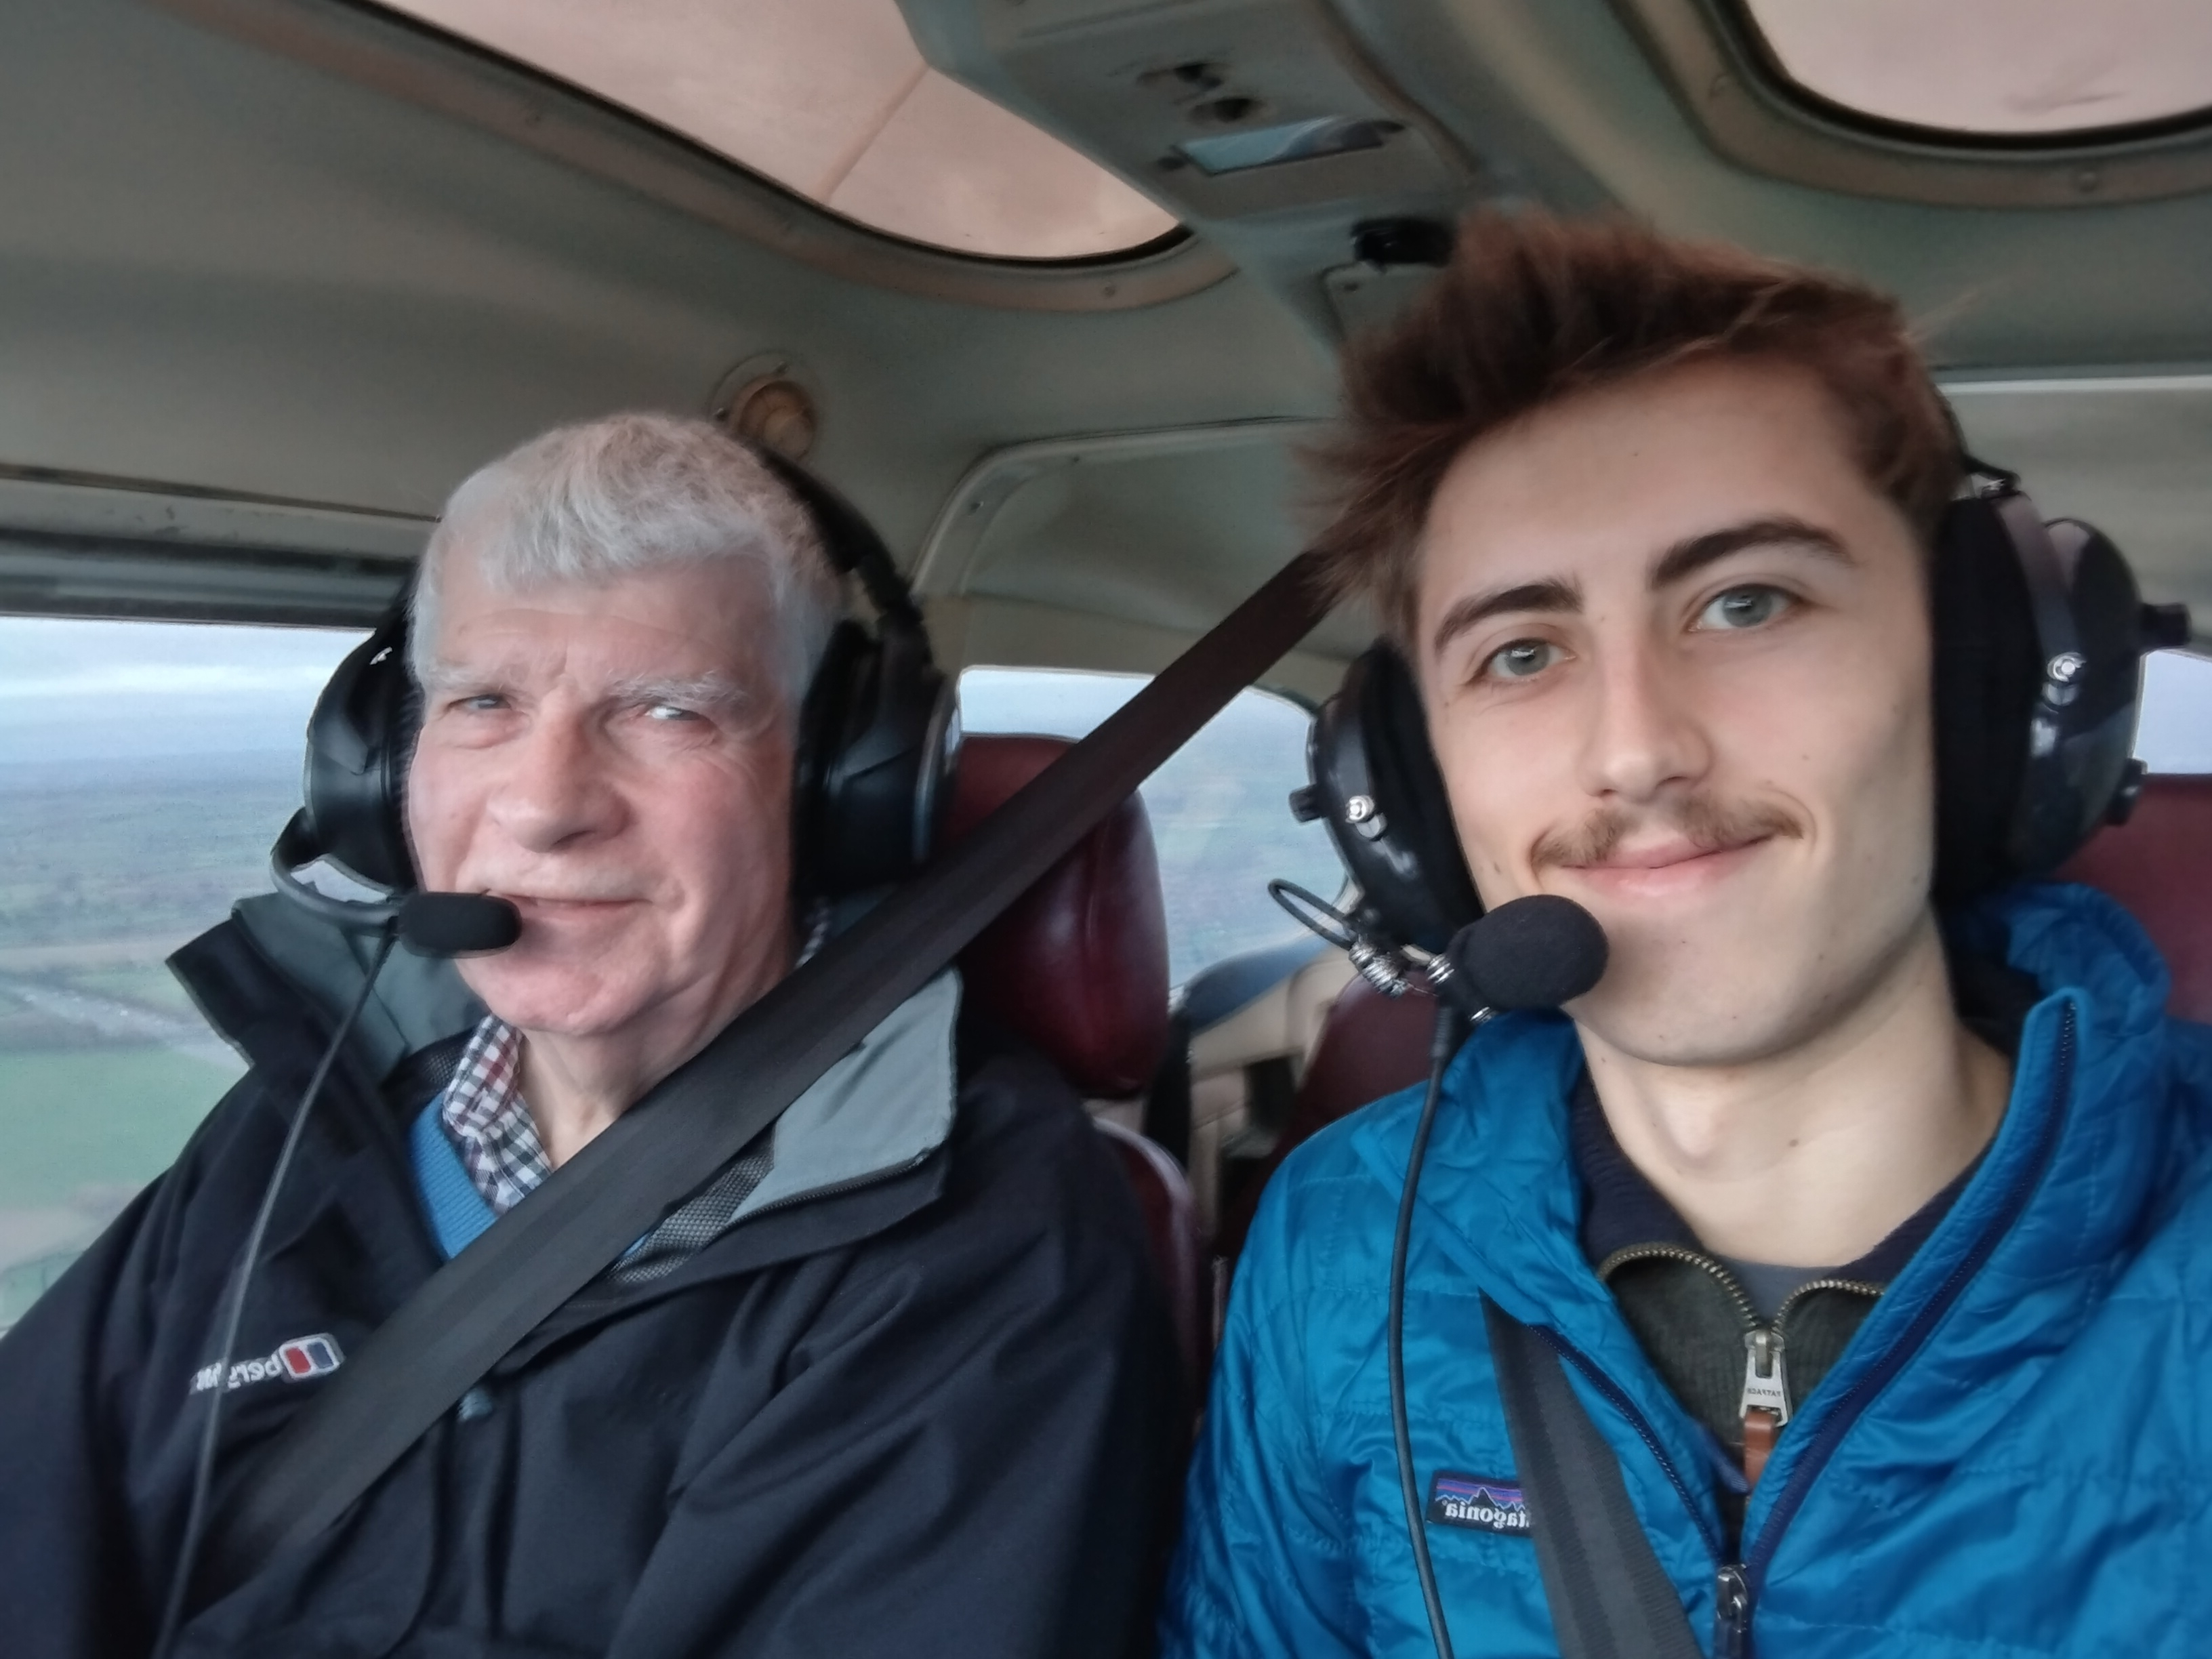
\includegraphics[scale = 0.08]{../document-resources/images/Aerial-selfie}
    \label{aerial-selfie}
    \caption{The client and student transiting Birmingham airspace.}
\end{figure}

The Coronavirus pandemic has increased the need for pilot refresher training, with the European Union Aviation Safety Agency (EASA) releasing guidelines on extra training for pilots and ground staff who are coming back from an extended break from work \cite{EASA-Training-Post-Covid}. Given the nature of the flight profession, pilots may not be able to attend regular in-person training if they are travelling. A system that offers online solo practice with no need for arranging an instructor could form part of a pilot’s continued skills practice.

\subsection{Existing Software}
Although limited by a lack of voice input support, two high quality and popular R/T practice applications are available online. Neither are open source, hence this project will involve developing many of the features found in these systems, with the addition of voice input.

Readability5 presents a simple interface which mimics the resources a student would have in the exam \cite{Readability5}, that being a radio, transponder, map, and kneeboard (a notepad often attached to a pilot's upper thigh). In each module the user is walked through a scenario in which, mimicking the actual exam, they must select the correct frequencies and modes on both the radio and transponder and transmit radio calls. Five modules which teach different aspects of R/T can be purchased, however the route used in each module is fixed, so once a module has been completed once, the next practice will be on the exact same route. Voice input is technically supported, but all speech is considered correct, so users can simply press the transmit button without saying anything and progress to the next state in the scenario.

Wilco Radio is a feature rich training system which provides many practice modes including mock tests \cite{Wilco-Radio}. Its interface shows much more information than that of Readability5, much of it being unnecessary for the exam. It also does not support the managing of radio and transponder frequencies and modes, which are part of the skills required to pass the R/T exam. Its fundamental flaw is the form of input it supports - users select from a set of predefined options given by the system to respond to each radio message. Despite this, it does provide extensive feedback on radio calls, and shows the user's progress metrics including the number of procedures practised, and the user's accuracy rate.
